\documentclass[12pt,twoside]{article}
\usepackage{amsmath, amssymb}
\usepackage{amsmath}
\usepackage[active]{srcltx}
\usepackage{amssymb}
\usepackage{amscd}
\usepackage{makeidx}
\usepackage{amsthm}
\usepackage{algpseudocode}
\usepackage{algorithm}
\usepackage{graphicx}
\usepackage[spanish]{babel}
\renewcommand{\baselinestretch}{1}
\graphicspath{{images/}}
\setcounter{page}{1}
\setlength{\textheight}{21.6cm}
\setlength{\textwidth}{14cm}
\setlength{\oddsidemargin}{1cm}
\setlength{\evensidemargin}{1cm}
\pagestyle{myheadings}
\thispagestyle{empty}
\markboth{\small{Pr\'actica 2. Alan, Josu\'e}}{\small{.}}
\date{}
\begin{document}
\centerline{\bf An\'alisis de Algoritmos, Sem: 2020-1, 3CV2, Pr\'actica 2, 28 de agosto}
\centerline{}
\centerline{}
\begin{center}
\Large{\textsc{Pr\'actica 2: Funciones Recursivas vs Iterativas}}
\end{center}
\centerline{}
\centerline{\bf {Alan Romero Lucero, Josué David Hern\'andez Ram\'irez}}
\centerline{}
\centerline{Escuela Superior de C\'omputo}
\centerline{Instituto Polit\'ecnico Nacional, M\'exico}
\centerline{$alanrl.escom@gmail.com, correo@alumno_2$}
\newtheorem{Theorem}{\quad Theorem}[section]
\newtheorem{Definition}[Theorem]{\quad Definition}
\newtheorem{Corollary}[Theorem]{\quad Corollary}
\newtheorem{Lemma}[Theorem]{\quad Lemma}
\newtheorem{Example}[Theorem]{\quad Example}
\bigskip
\textbf{Resumen:} Para esta pr\'actica de realiz\'o la comparaci\'on de dos algoritmos, uno recursivo y uno iterativo, para la resoluci\'on de un mismo problema.
{\bf Palabras Clave:} {\textit{algoritmo, complejidad, iterativo, recursivo}}
\section{Introducci\'on}
En el an\'alisis de algoritmos es muy com\'un encontrarnos con problemas que pueden ser resueltos con mas de un algoritmo, donde simplemente elegimos uno u otro. Sin embargo, en ocaciones la diferencia de aplicar un algoritmo u otro puede afectar severamente el tiempo de ejecuci\'on.

Considere la situaci\'on en la que hay un problema que resolver, se analizar y se llega a dos algoritmos que lo resuelven. Uno de los algoritmos es iterativo y el otro es recursivo, ¿Cual se deber\'ia implementar? Si el algoritmo recursivo es aparentemente mas f\'acil de implementar que el iterativo, ¿es buena idea implementarlo? Por lo anterior, es importante analizar estos casos, donde la diferencia entre un algoritmo recursivo e iterativo es crucial.
\section{Conceptos B\'asicos}
Para esta pr\'actica se implementaron los siguientes algoritmos para: encontrar la suceci\'on de fibonacci hasta el $n-esimo$ numero, de manera recursiva e iterativa; encontrar la suma de los cubos de los primeros $n$ n\'umeros.
\subsection{Sucesi\'on de Fibonacci}
La suceci\'on de fibonacci es la sucesi\'on de numeros tal que el $n-esimo$ elemento es igual a la suma de los dos elementos anteriores.
\subsubsection{Recursivo}
\begin{algorithmic}
    \Require n
    \State \textbf{fibonacci}$(n)$
    \If{$n=1$ or $n=2$}
        \State \textbf{return} 1
    \Else
        \State $a \longleftarrow \textbf{fibonacci(n-1)}$
        \State $b \longleftarrow \textbf{fibonacci(n-2)}$
        \State \textbf{return} $a+b$
    \EndIf
\end{algorithmic}
\subsubsection{Iterativo}
\begin{algorithmic}
    \Require n
    \State \textbf{fibonacci}$(n)$
    \State $fibo\longleftarrow1$
    \State $a\longleftarrow1$
    \State $b\longleftarrow0$
    \State $i\longleftarrow1$
    \For{$i < n$}
        \State $fibo\longleftarrow a+b$
        \State $b\longleftarrow a$
        \State $a\longleftarrow fibo$
    \EndFor
    \State \textbf{return} $fibo$
\end{algorithmic}

\subsection{Suma de los primeros $N$ cubos}
El algoritmo recursivo de este problema fue proporcionado para la practica. El algoritmo encuentra la suma de los primeros $n$ cubos.
\subsubsection{Recursivo}
\begin{algorithmic}
    \Require n
    \State \textbf{suma}$(n)$
    \If{$n=1$}
        \State \textbf{return} 1https://es.overleaf.com/project/5d66a9948a6668118730a11f
    \Else
        \State \textbf{return} $suma(n-1)+n\textsuperscript{3}$
    \EndIf
\end{algorithmic}
\subsubsection{Iterativo}
\begin{algorithmic}
    \Require n
    \State \textbf{suma}$(n)$
    \State $sum \longleftarrow 0$
    \State $i \longleftarrow1$
    \For{$i \leq n$}
        \State $sum \longleftarrow sum + i\textsuperscript{3}$
    \EndFor
    \State \textbf{return} $sum$
\end{algorithmic}
\section{Experimentaci\'on y Resultados}
La implementaci\'on de los algoritmos para fibonacci y la suma de los primeros cubos fue probada con valores aleatorios.
\subsection{Fibonacci}
\subsubsection{Iterativo}
Para empezar, para la sucesi\'on de fibonacci de manera iterativa se obtiene una complejidad de orden lineal. Esto puede ser mostrado gr\'aficamente por la figura 1. Se propone una funci\'on $g(n) = \frac{5}{2} n$.
\begin{figure}[ht]
    \centering
    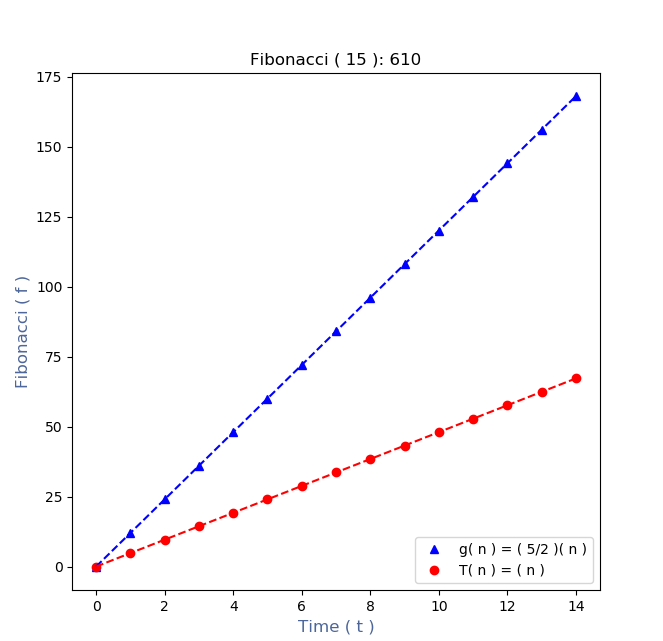
\includegraphics[width = 13cm,height = 6cm]{fibonacci_iterativo_grafica.png}
    \caption{Gr\'afica del algoritmo iterativo para la sucesi\'on de fibonacci}
    \label{fig:fibonacci_iterativo_graph}
\end{figure}

Revisando nuevamente el algoritmo, hace falta demostrar que su complejidad sea efectivamente de orden lineal, por lo que se hace su an\'alisis linea por linea.

\begin{algorithmic}
    \Require n
    \State \textbf{fibonacci}$(n)$
    \State $fibo\longleftarrow1$
    \State $a\longleftarrow1$
    \State $b\longleftarrow0$
    \State $i\longleftarrow1$
    \For{$i < n$}
        \State $fibo\longleftarrow a+b$
        \State $b\longleftarrow a$
        \State $a\longleftarrow fibo$
    \EndFor
    \State \textbf{return} $fibo$
\end{algorithmic}
\begin{figure}[ht]
    \centering
    \begin{tabular}{ |c|c|c| } 
         \hline
         \textbf{Linea/Constante de tiempo} & \textbf{Conteo} \\ 
         $c1$ & $1$ \\ 
         $c2$ & $1$ \\ 
         $c3$ & $1$ \\ 
         $c4$ & $1$ \\ 
         $c5$ & $n$ \\ 
         $c6$ & $n-1$ \\ 
         $c7$ & $n-1$ \\ 
         $c8$ & $n-1$ \\ 
         \hline
    \end{tabular}
    \caption{An\'alisis linea por linea del algoritmo iterativo para fibonacci}
    \label{fig:tabla_iterativo_fibo}
\end{figure}
\begin{figure}[ht]
    \centering
    \begin{equation}
        c\textsubscript{1}+c\textsubscript{2}+c\textsubscript{3}+c\textsubscript{4}+c\textsubscript{5}n+c\textsubscript{6}(n-1)+c\textsubscript{7}(n-1)+c\textsubscript{8}(n-1)
    \end{equation}
    \begin{equation}
        (c\textsubscript{1}+c\textsubscript{2}+c\textsubscript{3}+c\textsubscript{4})+c\textsubscript{5}n+c\textsubscript{6}n-c\textsubscript{6}+c\textsubscript{7}n-c\textsubscript{7}+c\textsubscript{8}n-c\textsubscript{8}
    \end{equation}
    \begin{equation}
        (c\textsubscript{5}+c\textsubscript{6}+c\textsubscript{7}+c\textsubscript{8})n+(c\textsubscript{1}+c\textsubscript{2}+c\textsubscript{3}+c\textsubscript{4}-c\textsubscript{6}-c\textsubscript{7}-c\textsubscript{8})
    \end{equation}
    \begin{equation}
        an+b
    \end{equation}
    \caption{C\'alculo de complejidad del algoritmo iterativo para fibonacci}
    \label{eq:demo_fibo_iterativo}
\end{figure}
El an\'alisis lleva a una expresi\'on $an+b$, por lo que su complejidad es de orden lineal $O(n)$. Finalmente, la funci\'on propuesta $g(n) \in O(n)$.
\begin{figure}[ht]
    \centering
    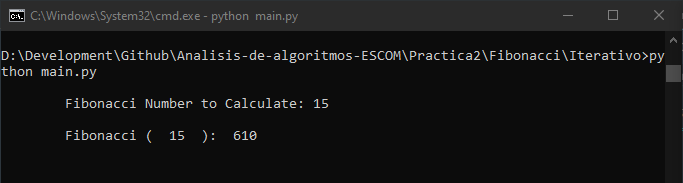
\includegraphics[width = 9cm]{fibonacci_iterativo_consola.png}
    \caption{Programa en ejecuci\'on de fibonacci de manera iterativa}
    \label{fig:fibonacci_iterativo}
\end{figure}
\subsubsection{Recursivo}
El algoritmo recursivo presenta una complejidad significativamente mayor al iterativo, como se puede ver en la gr\'afica (Figura 6).
\begin{figure}[ht]
    \centering
    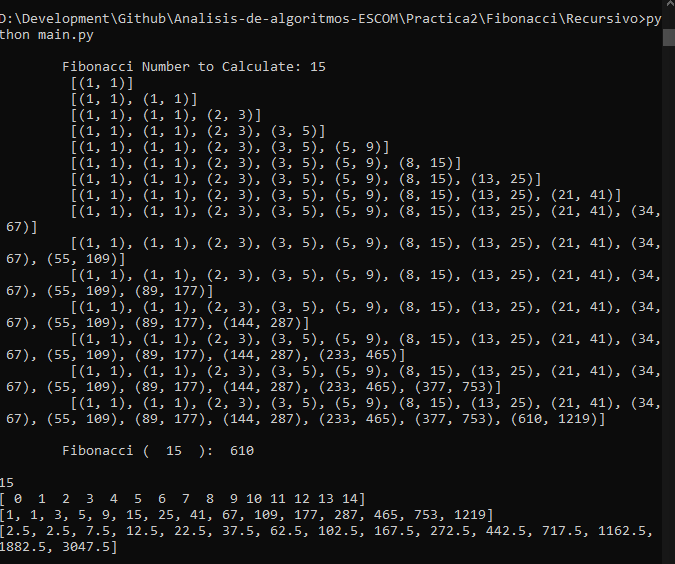
\includegraphics[width = 9cm]{fibonacci_recursivo_consola.png}
    \caption{Programa en ejecuci\'on de fibonacci de manera recursiva}
    \label{fig:fibonacci_recursiva}
\end{figure}
Es mas dificil hablar de la complejidad del algoritmo recursivo, tanto por su calculo como por su obtenci\'on de manera experimental. La complejidad de este algoritmo es propuesta como $g(n) = \frac{5}{2} \phi^n$, donde $\phi$ es el conocido numero \'aureo, el cual esta definido como:
\begin{figure}[ht]
    \centering
    \begin{equation}
        \phi = \frac{1 + \sqrt{5}}{2} = 1.6180
    \end{equation}
    \caption{Definici\'on del numero \'aureo}
    \label{fig:phi}
\end{figure}
\begin{figure}[ht]
    \centering
    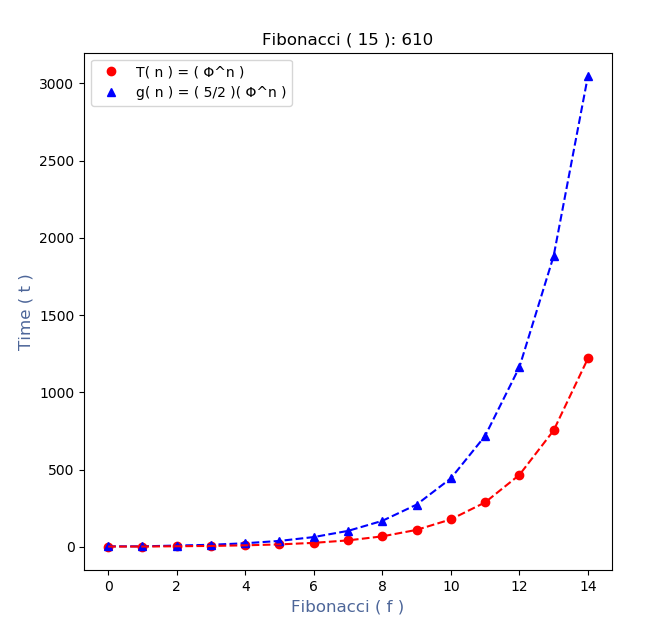
\includegraphics[width = 13cm,height = 8cm ]{fibonacci_recursivo_grafica.png}
    \caption{Gr\'afica de la complejidad del algoritmo recursivo para la sucesi\'on de fibonacci}
    \label{fig:fibonacci_recursiva_grafica}
\end{figure}

Finalmente, $g(n) = \frac{5}{2} \phi^n \in O(\phi^n)$. Para terminar la secci\'on, cabe destacar que, efectivamente, en el caso del algoritmo recursivo para la suceci\'on de fibonacci el tiempo de ejecuci\'on creci\'o much\'isimo con numeros relativamente mas grandes.

\subsection{Suma de los primeros $N$ cubos}
A diferencia de los algoritmos de fibonacci, en la implementaci\'on de estos algoritmos no hay una diferencia en el orden de complejidad. Ambos algoritmos tienen una complejidad propuesta $g(n) = \frac{5}{2} n$. Finalmente, para la complejidad de ambos algoritmos, $g(n) = \frac{5}{2} n \in O(n)$
\subsubsection{Iterativo}
\begin{figure}[ht]
    \centering
    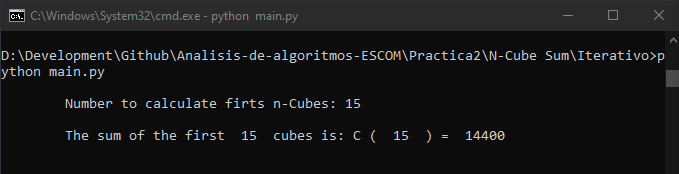
\includegraphics[width = 9cm]{cubico_iterativo_consola.png}
    \caption{Programa en ejecuci\'on del algoritmo iterativo para la suma de los n primeros cubos}
    \label{fig:n_cubos}
\end{figure}
\begin{figure}[ht]
    \centering
    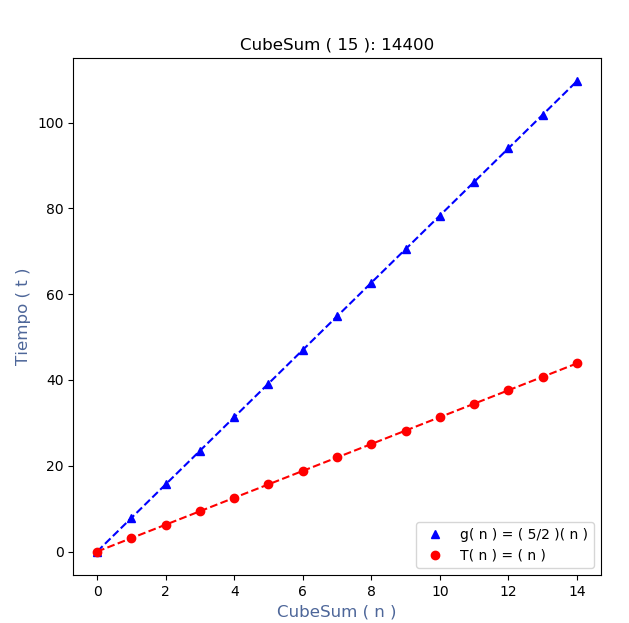
\includegraphics[width = 13cm,height = 8cm ]{cubico_iterativo_grafica.png}
    \caption{Gr\'afica de complejidad, algoritmo de suma de los n primeros cubos}
    \label{fig:n_cubos_graf}
\end{figure}
\subsubsection{Recursivo}
\begin{figure}[ht]
    \centering
    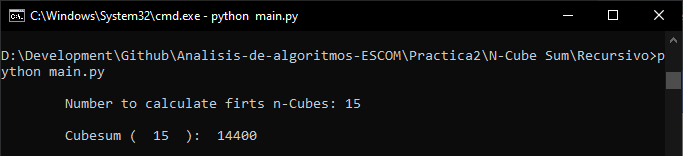
\includegraphics[width = 9cm]{cubico_recursivo_consola.png}
    \caption{Programa en ejecuci\'on del algoritmo recursivo para la suma de los n primeros cubos}
    \label{fig:n_cubos_rec}
\end{figure}
\begin{figure}[ht]
    \centering
    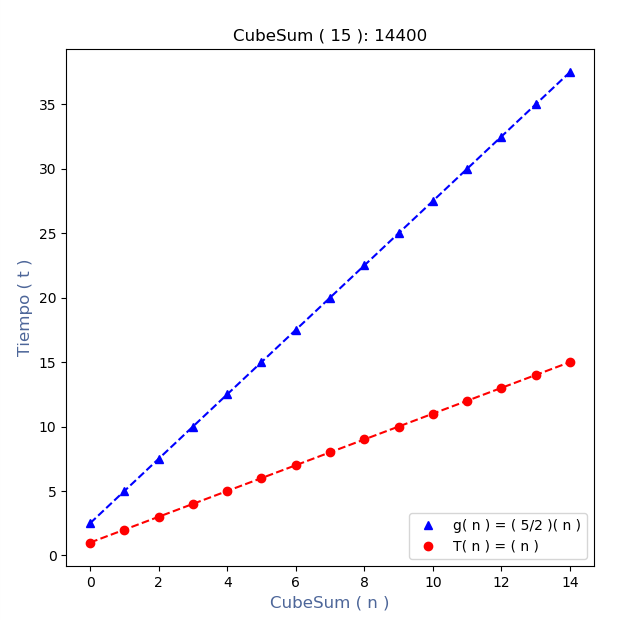
\includegraphics[width = 13cm,height = 8cm ]{cubico_recursivo_grafica.png}
    \caption{Gr\'afica de complejidad, algoritmo de suma de los n primeros cubos de forma recursiva}
    \label{fig:n_cubos_rec_graf}
\end{figure}

\newpage
\vfill
\clearpage
\section{Conclusiones}
La ejecuci\'on de los programas, en el caso de los algoritmos para la sucesi\'on de fibonacci, se hizo una prueba con la suceci\'on hasta elemento numero 50 con el recursivo. Como es evidente, dada la complejidad del algoritmo, nunca termino de ejecutarse el programa, o al menos no esperamos lo suficiente para que se terminara de ejecutar.

\textit{Alan Romero Lucero}. Es interesante ver como pueden variar mucho la complejidad de un algoritmo dependiendo si es iterativo o recursivo. Es f\'acil pensar que la diferencia siempre va a existir, haci\'endolo mas complejo o simple, sin embargo, en el ejemplo del algoritmo para la suma de los primeros n cubos la elecci\'on de uno de los dos tipos de algoritmos es poco trascendente. Aun as\'i, existen casos completamente contrarios, como la sucesi\'on de fibonacci donde la elecci\'on entre iterativo y recursivo es crucial.

\textit{Josu\'e David Hern\'andez Ram\'i rez}. En esta pr\’actica lo que logre al desarrollar los algoritmos fue entender mas como funcionan los algoritmos recursivos e iterativos, sabiendo mas a fondo que el coste computacional varia dependiendo de como este desarrollado un algoritmo, puesto que, como vimos en esta pr\’actica el algoritmo de Fibonacci es mejor desarrollarlo de manera iterativa, ya que su coste computacional es lineal a comparaci\’on de su desarrollo de manera recursiva, puesto que, al ser desarrollado de esta manera su coste se elevaba a medida que calculaba m\’as y m\’as los números de Fibonacci. Result\’o algo gracioso, puesto que mi computadora tard\’o toda una noche en cumplir el objetivo de calcular los primeros 50 números de la sucesi\’on de Fibonacci.\\
Por otro lado, en la suma de los primeros N cubos su desarrollo en iterativo y recursivo no cambia su complejidad y por ende su coste computacional siendo que el peor caso vale lo mismo que en su mejor caso.
 

\section{Anexo}
Se proporciono el siguiente algoritmo para su resolucion.
\begin{figure}[ht]
    \centering
    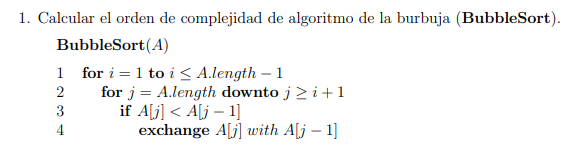
\includegraphics{anexo_2.png}
    \caption{Algoritmo de ordenamiento burbuja}
    \label{fig:bubble_sort}
\end{figure}
\begin{center}
\begin{tabular}{ | c | c | c | } 
 \hline
 \textbf{Linea/Constante de tiempo} & \textbf{Conteo} \\ 
 $c1$ & $n$ \\
 $c2$ & $\sum_{j=1}^{n} j$ \\
 $c3$ & $\sum_{j=1}^{n} j$ \\
 $c4$ & $\sum_{j=1}^{n} j$ \\
 \hline
\end{tabular}
\end{center}
\begin{figure}
    \centering
    \begin{equation}
        c1n+c2(\sum_{i=1}^{n}( j)+c3(\sum_{i=1}^{n} j)+c4(\sum_{i=1}^{n} (j)
    \end{equation}
    \begin{equation}
        n(c1)+\frac{(n^2)+ n}{2}(c2+c3+c4)
    \end{equation}
    \begin{equation}
        c(2.5n^2 + 1.5n)
    \end{equation}
    \label{eq:desarrollo_complejidad}
\end{figure}
\newpage
\vfill
\clearpage
\section{Bibliograf\'ia}
"Notaci\'on O may\'uscula", class notes for An\'alisis de Algoritmos, ESCOM-IPN, Verano 2019.
\end{document}
